\subsection{Human to Humanoid Robot Kinematic Mapping}\label{sec:sec:mocap}

Motion capture (MoCap) systems are commonly used to record high degree of freedom human motion.  
Athletic trainers in baseball, football and cycling use motion capture to analyze and improve throwing and lower limb motions\cite{Fleisig1996,barrentiine1998,Mochizuki1998,Akira1999}.
MoCap systems are also used to generate human-like motions and map those motion to humanoid robots\cite{1545060,Polland2002}.  
Fig.~\ref{fig:mocap-joints} shows the Hubo's kinematic structure (left) and the human (MoCap) kinematic structure(left).
The human has 3-DOF at each joint while the humanoid robot has limited DOF at each corresponding joint.
Some of the challenges in mapping between the human kinematic structure (from MoCap) to a humanoid robot's kinematic structure are:

\begin{itemize}
	\item The difference in the total degree of freedom (DOF). 
	\item	The difference in the kinematics descriptions. 
	\item	The different Kinematic constraints.
\end{itemize}

Stefan et. al.\cite{5756898} uses an intermediate model (Master Motor Map) to decouple motion capture data for further post-processing tasks. 
Our approach is to: 
a) Chose a set MoCap model.  
b) Preform motions where the pitch motions are decoupled (roll and yaw stays constant), avoids singularities and robot joint position limitations.  
c) Combine joint values for near by joints (reduce the model to the same DOF as the robot).  
d) Some tests require the addition of static offsets to joints to ensure the zero-moment-point (ZMP) criteria is satisfied as stated in Section~\ref{sec:sec:balance}

\begin{figure}[t]
  \centering
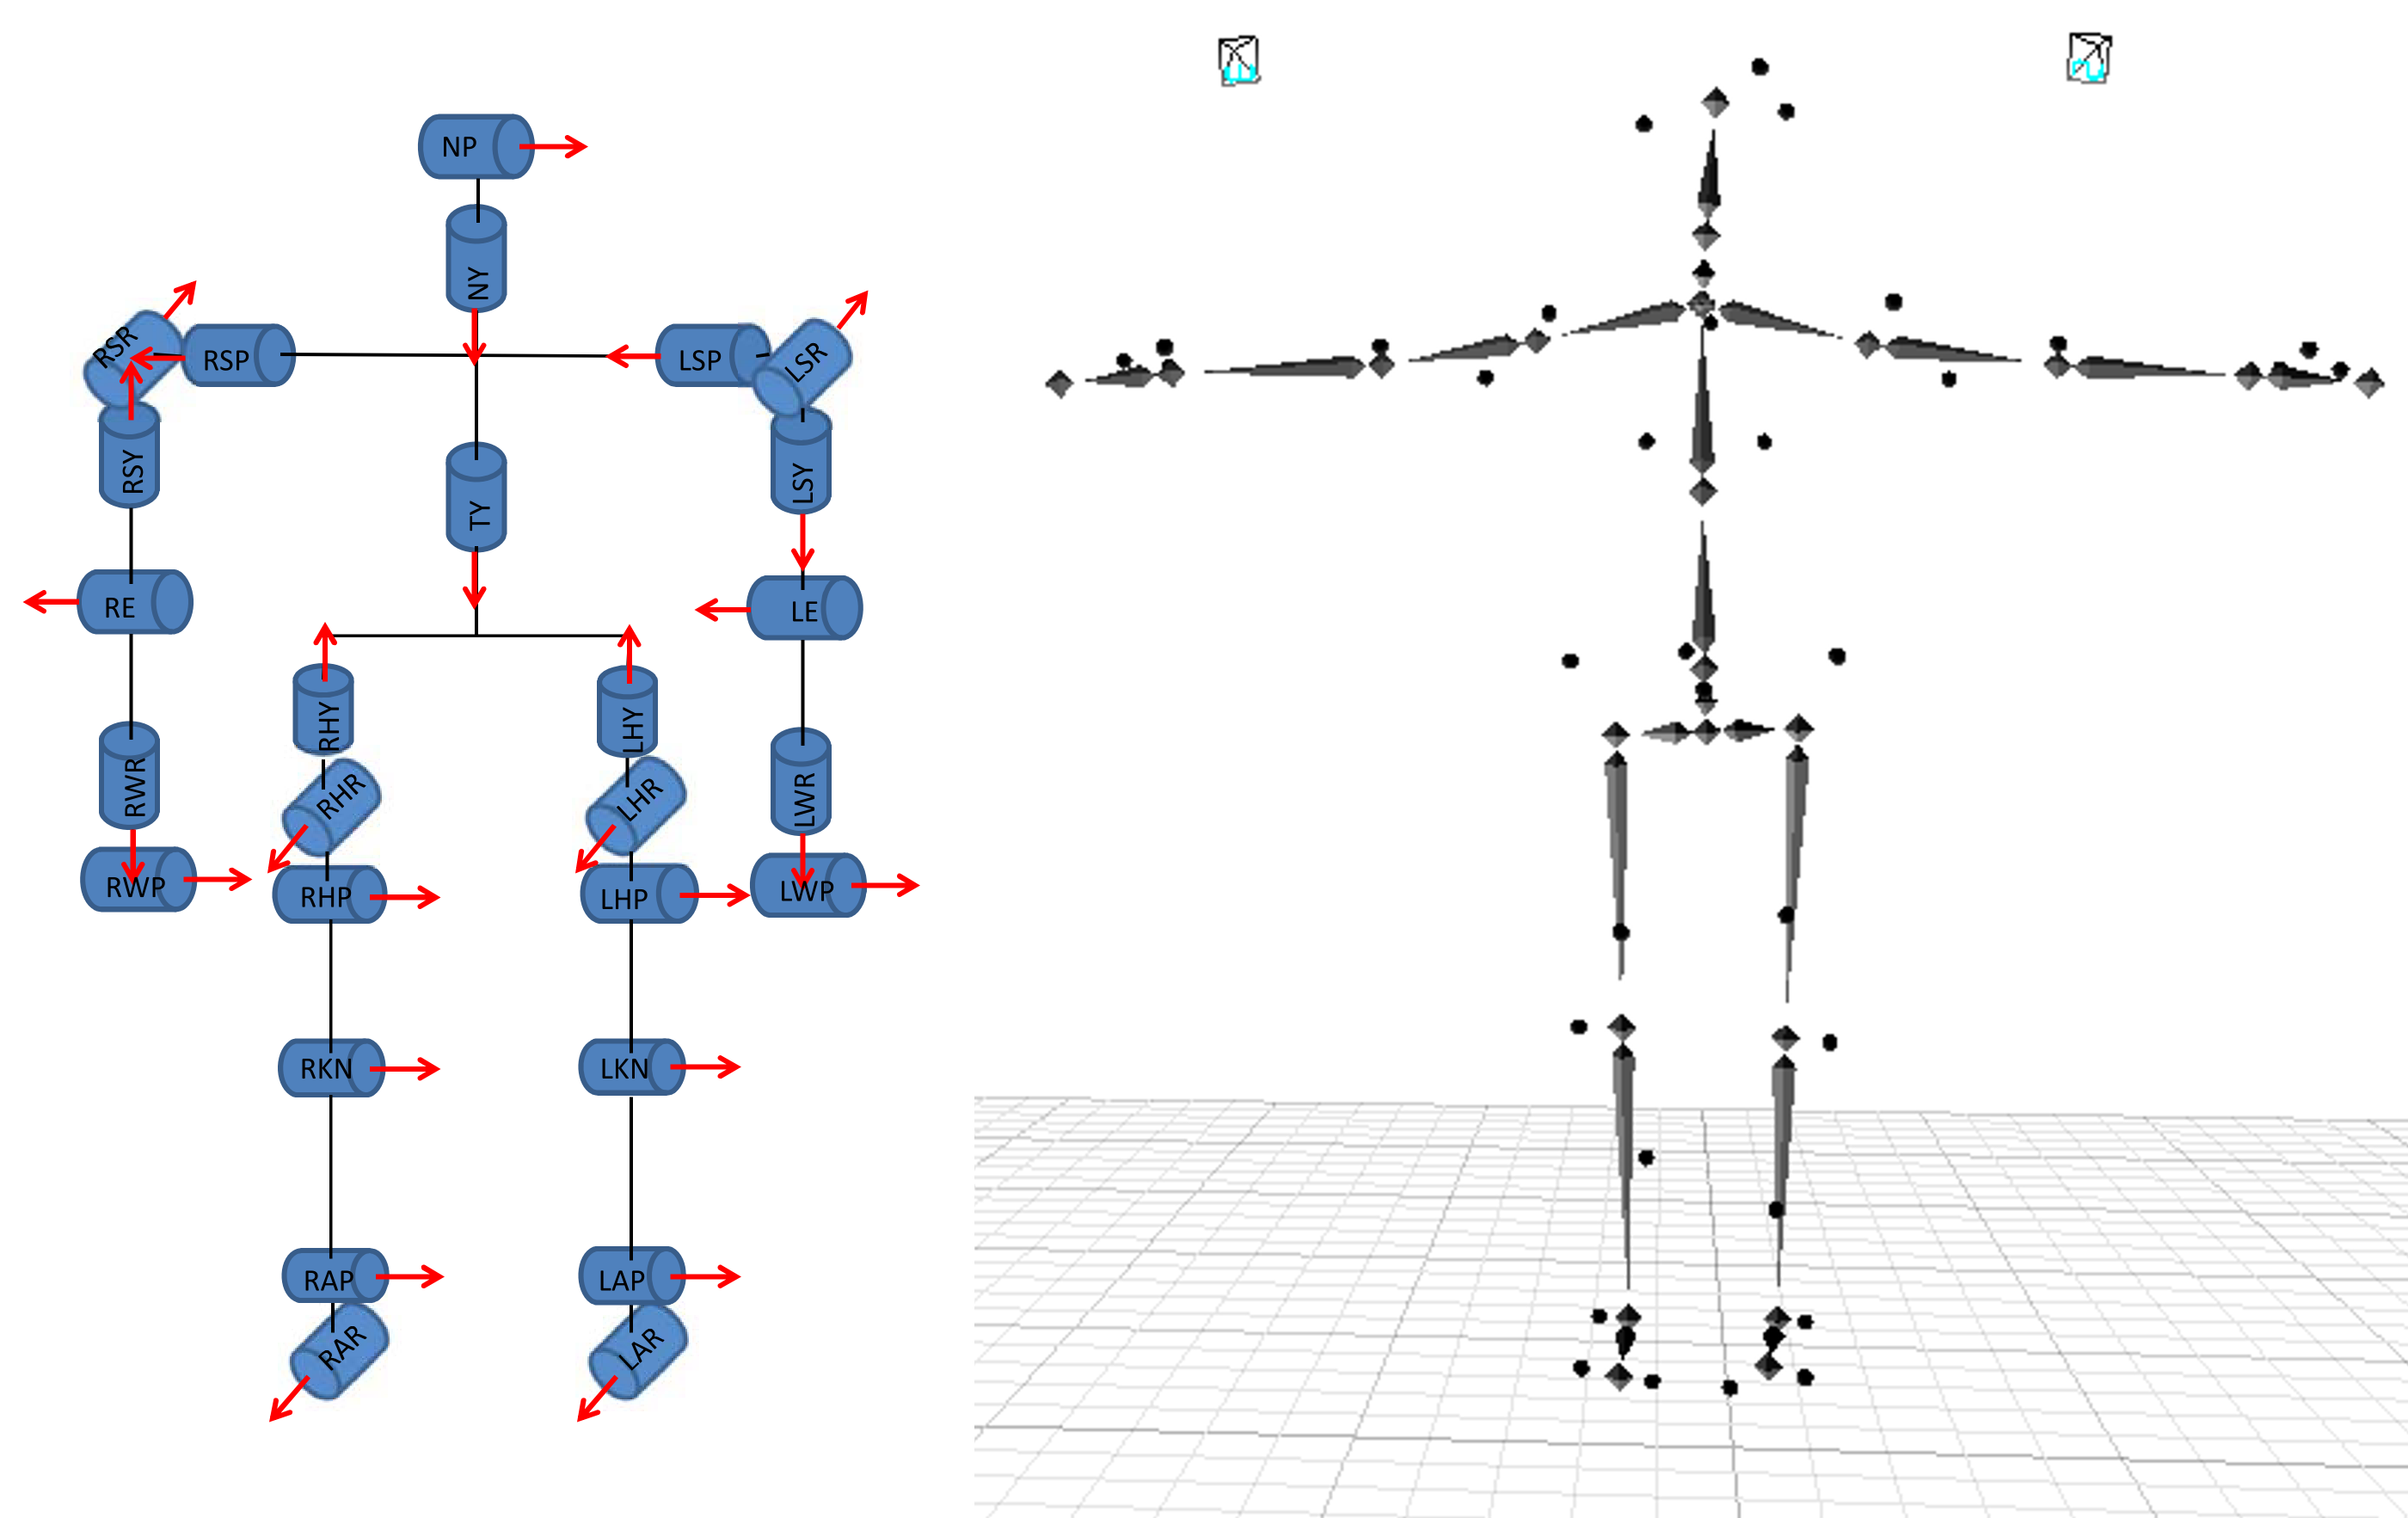
\includegraphics[width=1.0\columnwidth]{./pix/mocapJoints.png}  \caption{Left: Jaemi Hubo joint order and orientation using right hand rule.  Right: Motion capture model of human figure}
  \label{fig:mocap-joints}
\end{figure}



To test this method we used a human subject to throw a ball using upper and lower body movements.  
All motions were in the sagittal plane to keep pitch joints decoupled.  
To avoid the robot's joint limit of $\pm180^o$ an underhand throwing motion was used.
Fig.~\ref{fig:mocap-underhand} shows the human throwing the ball and the robot throwing the ball to the mapped motion of the human.

\begin{figure}[t]
  \centering
\includegraphics[width=1.0\columnwidth]{./pix/mocap/throwmocap3.png}
%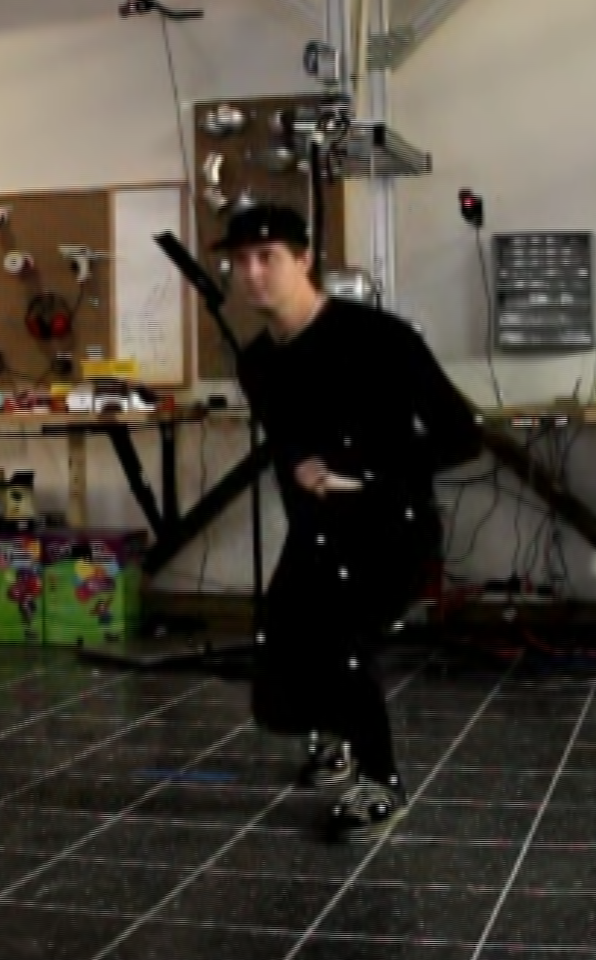
\includegraphics[width=0.33\columnwidth]{./pix/mocap/1a.png}
%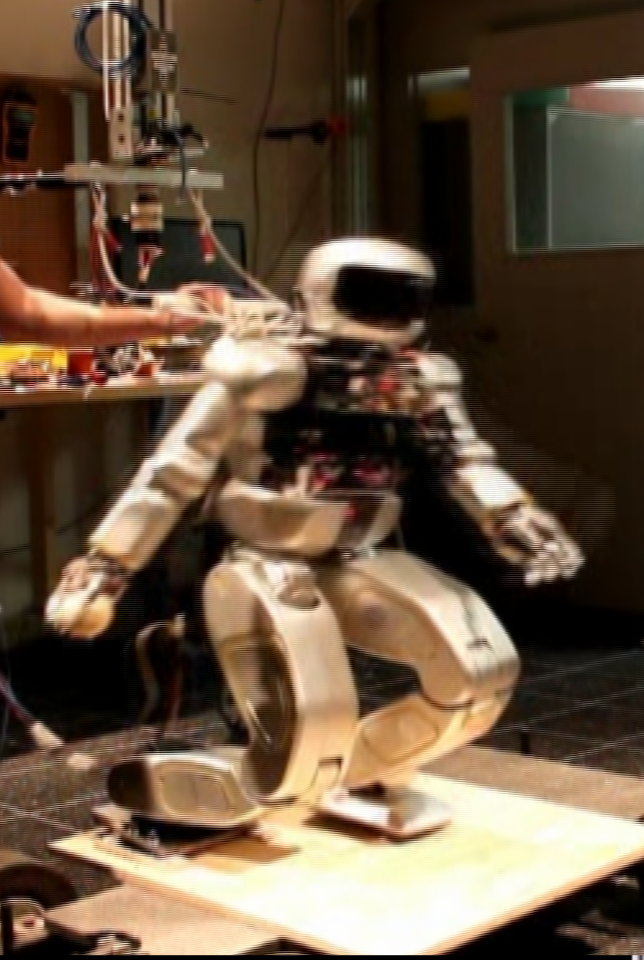
\includegraphics[width=0.33\columnwidth]{./pix/mocap/1b.png}
%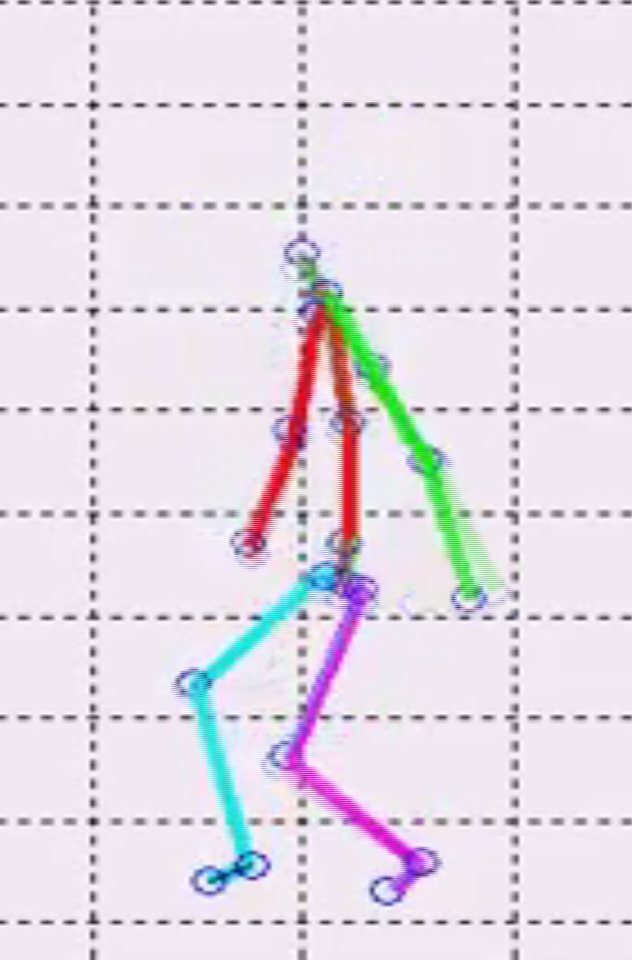
\includegraphics[width=0.33\columnwidth]{./pix/mocap/1c.png} 
%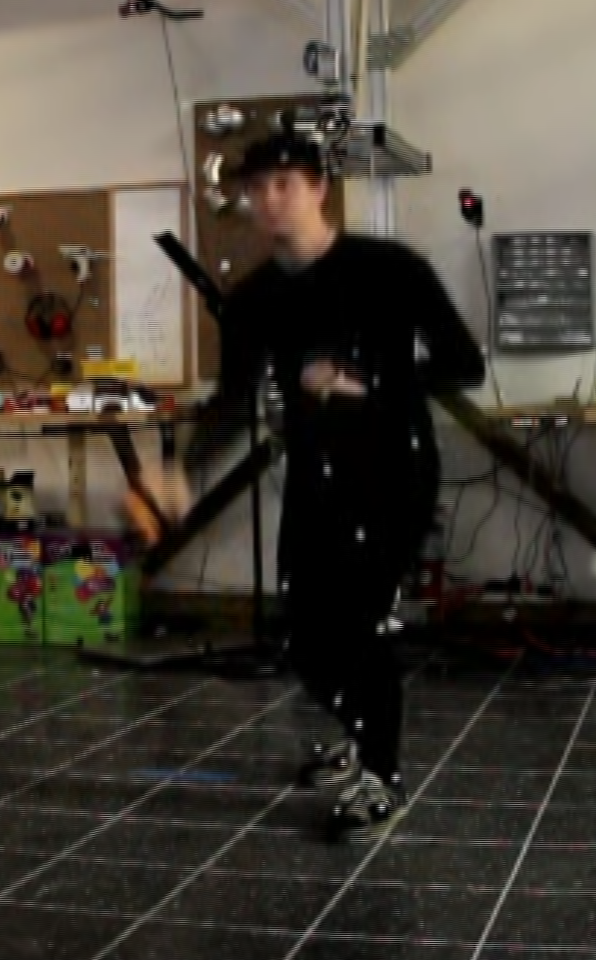
\includegraphics[width=0.33\columnwidth]{./pix/mocap/2a.png}
%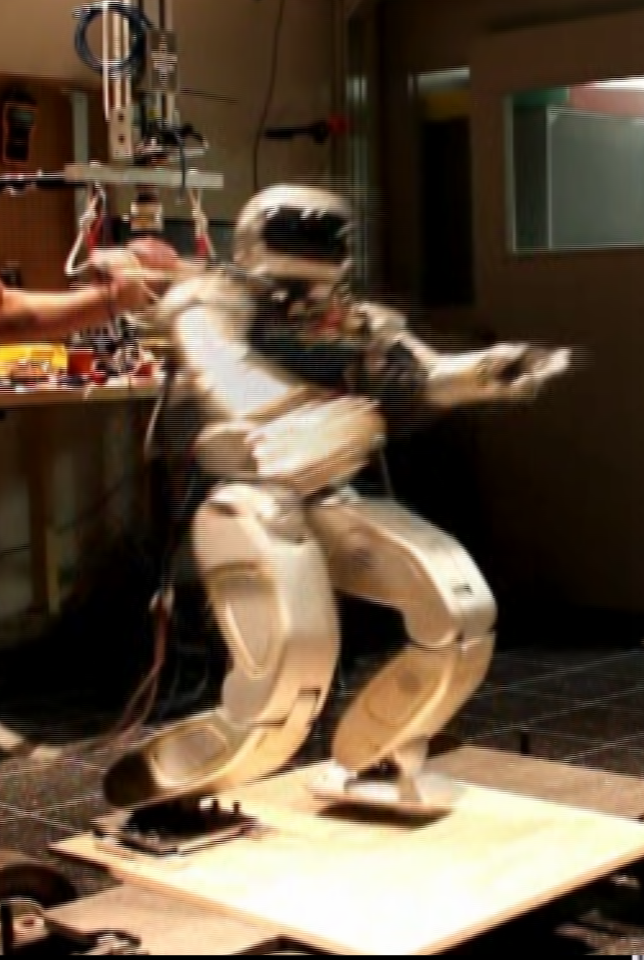
\includegraphics[width=0.33\columnwidth]{./pix/mocap/2b.png}
%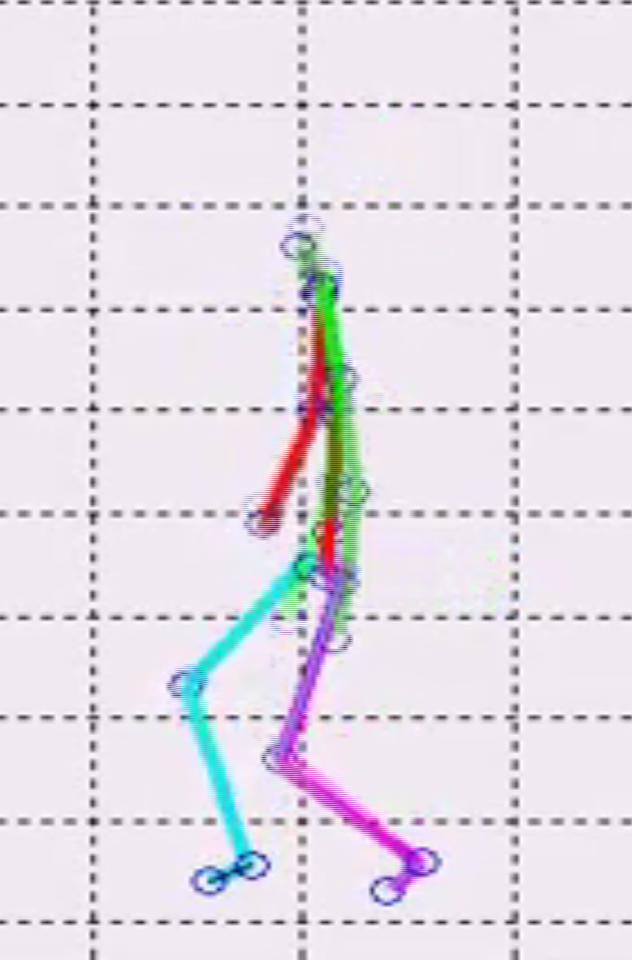
\includegraphics[width=0.33\columnwidth]{./pix/mocap/2c.png} 
%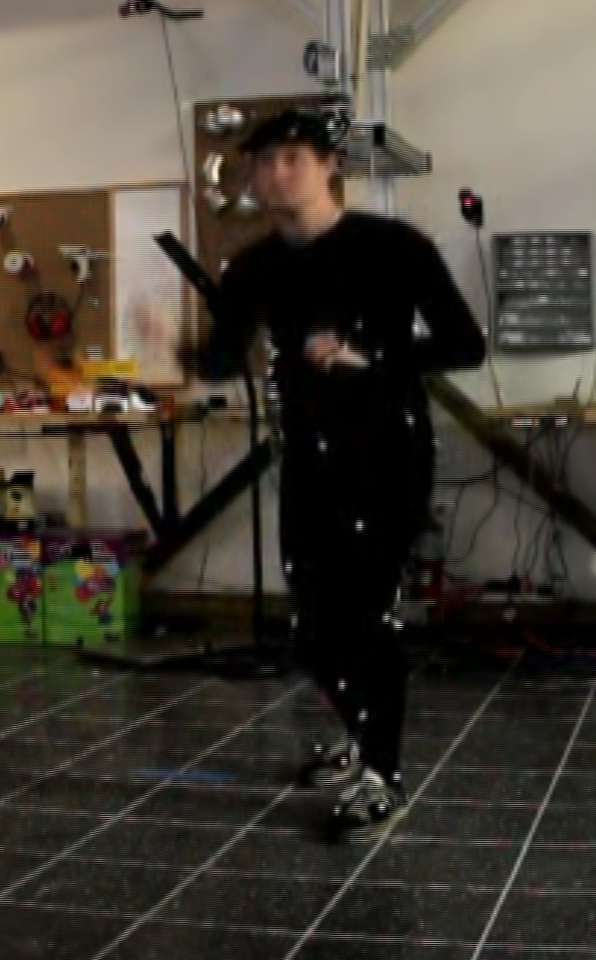
\includegraphics[width=0.33\columnwidth]{./pix/mocap/3a.png}
%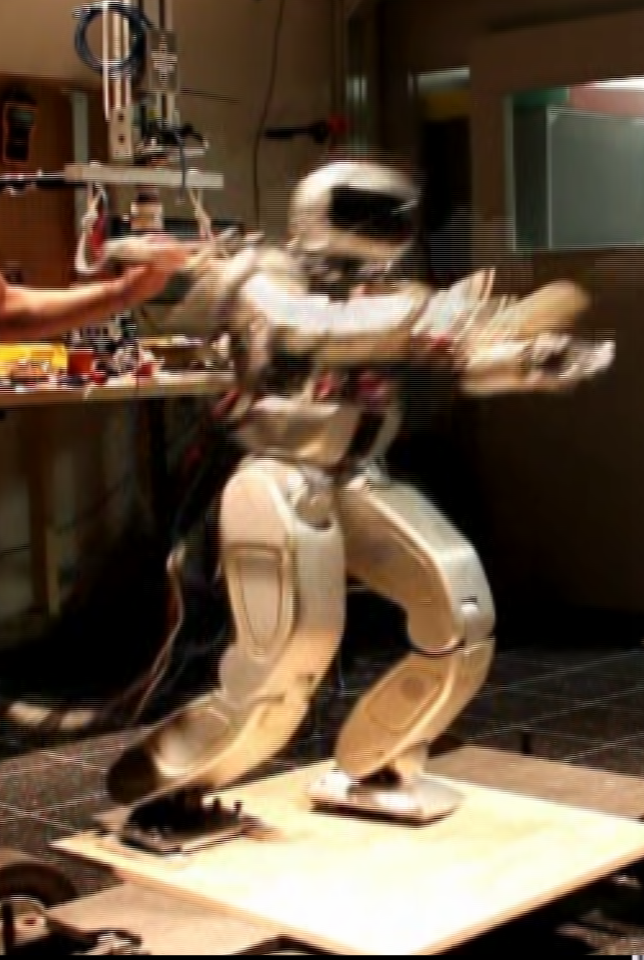
\includegraphics[width=0.33\columnwidth]{./pix/mocap/3b.png}
%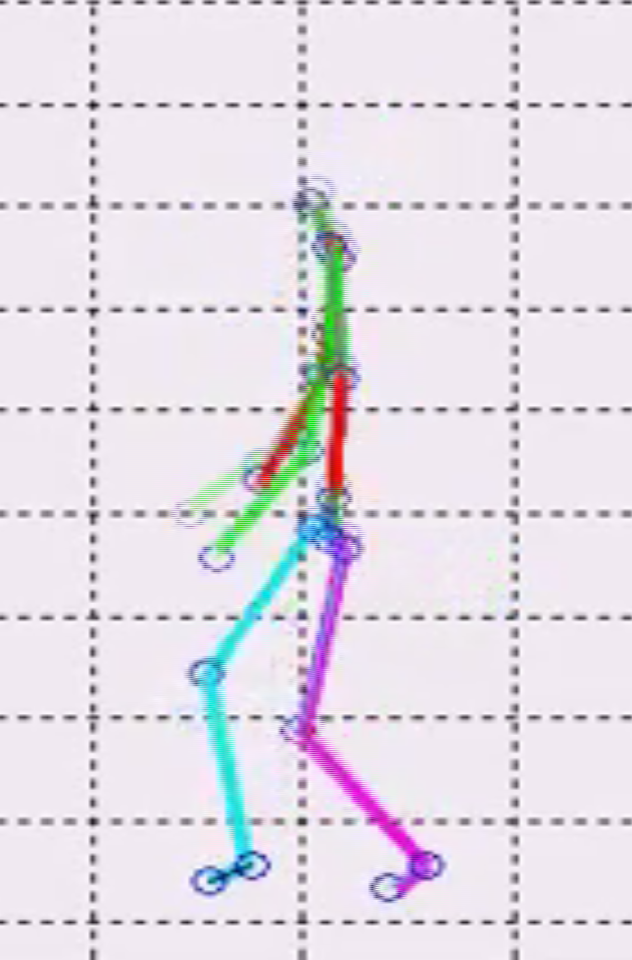
\includegraphics[width=0.33\columnwidth]{./pix/mocap/3c.png} 
%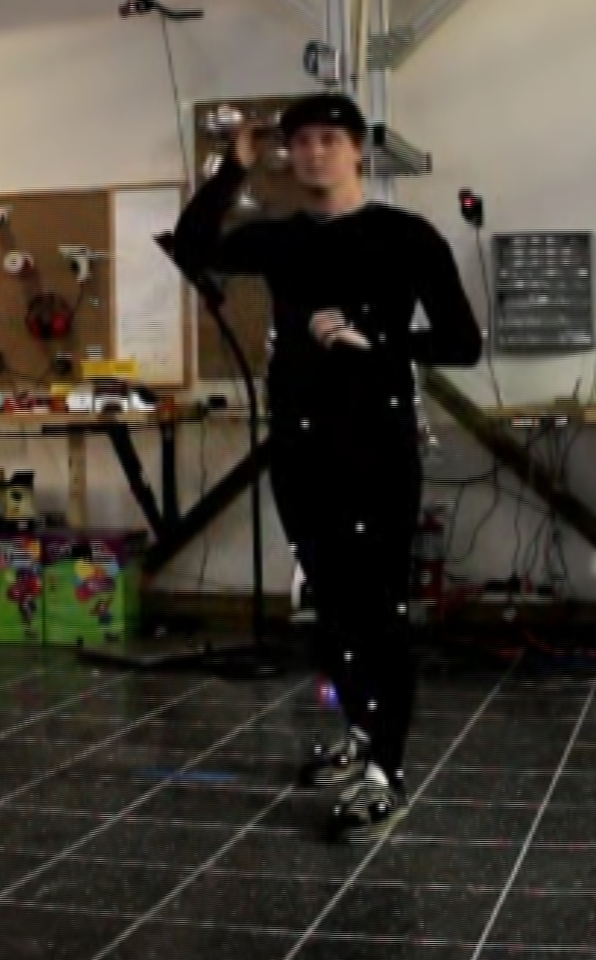
\includegraphics[width=0.33\columnwidth]{./pix/mocap/4a.png}
%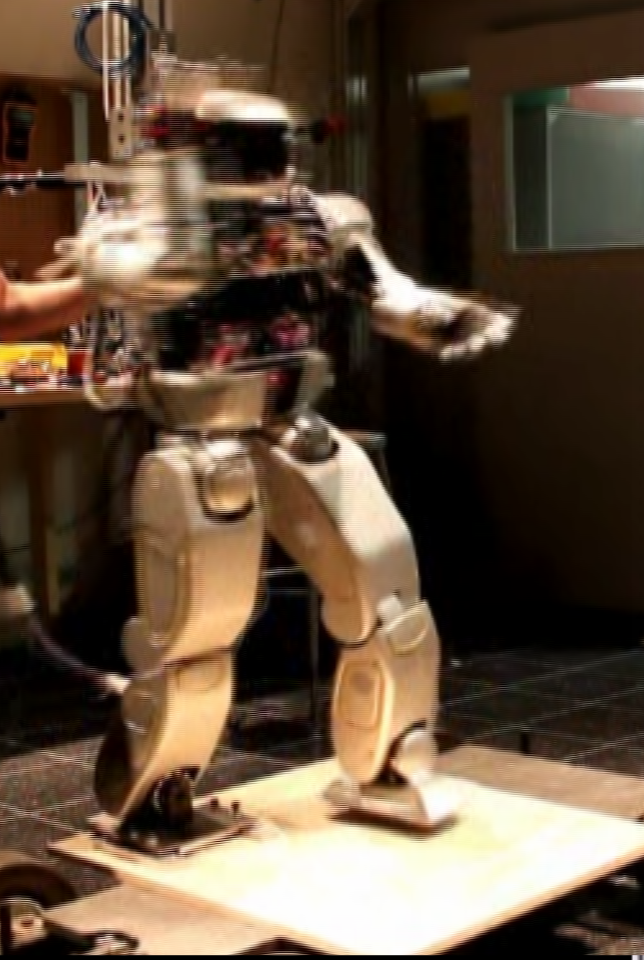
\includegraphics[width=0.33\columnwidth]{./pix/mocap/4b.png}
%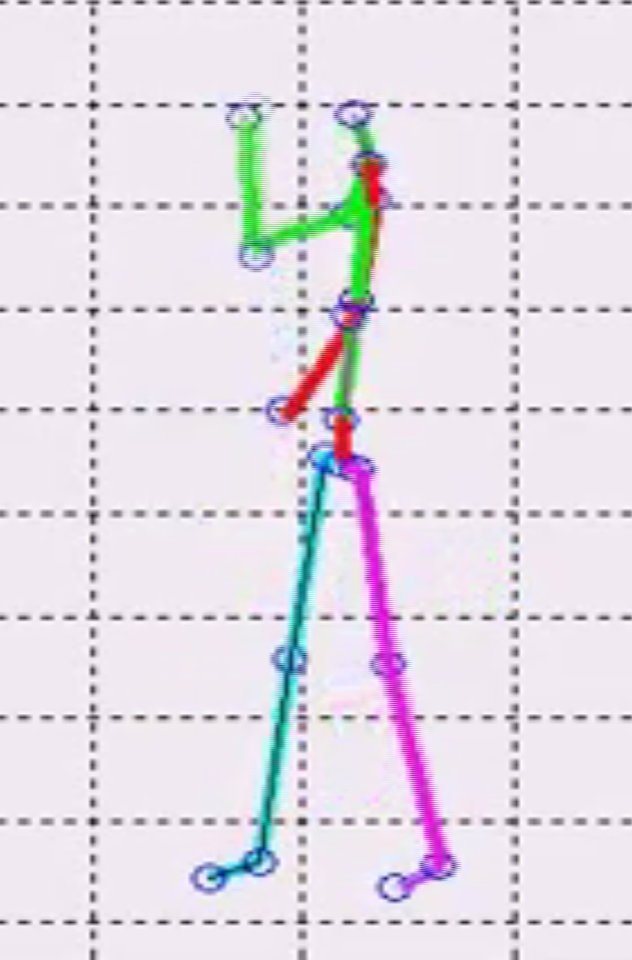
\includegraphics[width=0.33\columnwidth]{./pix/mocap/4c.png} 
  \caption{Left: Human frame by frame throwing underhand in sagittal plane.  Right: Throwing motion mapped to humanoid robot.}
  \label{fig:mocap-underhand}
\end{figure}

To ensure balance throughout the motion the balance controller as described in Section~\ref{sec:sec:balance} was applied and the static ZMP criteria was checked for the entire trajectory.
The human subject threw the ball approximately eight feet (244cm).  
The mapping of the latter motion caused the robot to throw the ball approximately five feet (152cm).
The discrepancy comes from the proportional difference in limb length from the human to the robot.
A side by side video of the human and the robot throwing the ball is available for viewing on the this papers's homepage\footnote{MoCap to Robot (Video): http://danlofaro.com/Humanoids2012/\#mocap}.




